\documentclass{article}
\usepackage [spanish] {babel} 
\usepackage{graphicx} 
 
\title{Tarea 3 Redes}
 
\author{Vicente Garc\'ia Huidobro}
 
\date{}
 
 
\begin{document}

\maketitle

 \begin{enumerate}
\item Investigac\'ion del porque de los paquetes y sus rutas \\
El dise\~no del protocolo IP se realiz\'o presuponiendo que la entrega de los paquetes de datos ser\'ia no confiable. Por ello, IP tratar\'a de realizarla del mejor modo posible, mediante t\'ecnicas de encaminamiento, sin garant\'ias de alcanzar el destino final pero tratando de buscar la mejor ruta entre las conocidas por la m\'aquina que est\'e usando IP.\\
Los datos en una red basada en IP son enviados en bloques conocidos como paquetes o datagramas los cuales en el protocolo IP son lo mismo. En particular, en IP no se necesita ninguna configuraci\'on antes de que un equipo intente enviar paquetes a otro con el que no se hab\'ia comunicado antes.\\
IP provee un servicio de datagramas no fiable, tambi\'en llamado el ``mejor esfuerzo" donde lo intentara hacer lo mejor posible, pero sin garant\'ia. IP no provee ningún mecanismo para determinar si un paquete alcanza o no su destino y únicamente proporciona seguridad de sus cabeceras y no de los datos transmitidos.\\
En comunicaciones, el enrutamiento es el mecanismo por el que en una red los paquetes de informaci\'on se hacen llegar desde su origen a su destino final, siguiendo un camino o ruta a trav\'es de la red. En una red grande o en un conjunto de redes interconectadas el camino a seguir hasta llegar al destino final puede suponer transitar por muchos nodos intermedios.\\
Asociado al encaminamiento existe el concepto de m\'etrica, que es una medida de lo ``bueno" que es usar un camino determinado. La m\'etrica puede estar asociada a distintas magnitudes: distancia, coste, retardo de transmisi\'on, n\'umero de saltos, etc., o incluso a una combinaci\'on de varias magnitudes. Si la m\'etrica es el retardo, es mejor un camino cuyo retardo total sea menor que el de otro. Lo ideal en una red es conseguir el encaminamiento \'optimo, tener caminos de distancia o coste, o retardo, o la magnitud que sea, seg\'un la m\'etrica m\'inimos. T\'ipicamente el encaminamiento es una funci\'on implantada en la capa 3.

\item ?`C\'omo viajan los paquetes de un continente a otro?\\
Internet trabaja seg\'un el esquema cliente/servidor, donde la computadora utilizada para navegar la Red es el cliente y las que proveen archivos y servicios son servidores o hosts. El intercambio de datos entre clientes y servidores se produce bajo las regulaciones de la suit de protocolos TCP/IP.\\ 
Todas las computadoras conectadas a la Red son identificadas mediante una direcci\'on IP consistente en cuatro grupos de n\'umeros separados por puntos. Por ejemplo, 198.112.168.223 es una direcci\'on IP. En general el primer grupo de n\'umero identifica la red a la que la m\'aquina est\'a conectada y el \'ultimo grupo de n\'umeros identifica a la propia m\'aquina.\\ 
Los datos intercambiados entre el cliente y el servidor son divididos en pequeños paquetes que viajan por la Red independientemente unos de los otros. Cada paquete incluye la direcci\'on IP del remitente y del destinatario, de manera que los intermediarios puedan dirigirlos a su destino sin mayores dificultades. Utilizando su sistema de direcciones, el protocolo IP es el encargado de que los paquetes lleguen a su destino. Teniendo en cuenta que el estado de la Red cambia continuamente y que los intermediarios deciden la ruta de los paquetes de acuerdo al estado de la Red en el instante en que los reciben, es usual que no todos los paquetes componentes de un mensaje sigan el mismo camino, lo que implica que no necesariamente llegaran al destinatario en el mismo orden en que los emiti\'o el remitente.\\ 
El protocolo TCP es el encargado de dividir los mensajes en paquetes, numerarlos, enviarlos a su destinatario, asegurarse de que llegan sin errores, y recomponer el mensaje ordenando los paquetes seg\'un la numeraci\'on de env\'io. TCP se encarga tambi\'en de pedirle al remitente que vuelva a enviar aquellos paquetes que llegaron al destinatario con errores.

\item Lista de enlaces internacionales que tiene Chile para conectarse a Internet\\
\begin{itemize}
\item United States	Mountain View	37.419205	-122.0574	72.14.234.41	(None)	3	459	9196
\item United States	Mountain View	37.419205	-122.0574	72.14.232.86	(None)	5	47	0
\item United States	Mountain View	37.419205	-122.0574	173.194.42.207	scl03s05-in-f15.1e100.net.	5	268	0
\item Spain	(Unknown)	40.0	-4.0	84.16.11.214	Hu0-4-0-0-GRTSCLOE1.red.telefonica-wholesale.net.	37	45	10665
\item Spain	(Unknown)	40.0	-4.0	5.53.3.75	Hu0-7-0-0-grtmiabr5.red.telefonica-wholesale.net.	19	65	0
\item Spain	(Unknown)	40.0	-4.0	94.142.123.5	Te0-2-0-4-grtmiana4.red.telefonica-wholesale.net.	3	45	0
\item United States	Wilmington	39.735107	-75.6684	63.243.152.45	ix-4-3-1-0.tcore1.MLN-Miami.as6453.net.	4	44	5944
\item United States	(Unknown)	38.0	-97.0	66.198.154.177	if-7-2.tcore1.AEQ-Ashburn.as6453.net.	3	526	1854
\item United States	(Unknown)	38.0	-97.0	216.6.87.1	if-2-2.tcore2.AEQ-Ashburn.as6453.net.	39	520	0
\item United States	(Unknown)	38.0	-97.0	216.6.87.138	if-11-2.tcore2.NJY-Newark.as6453.net.	16	243	0
\item United States	(Unknown)	38.0	-97.0	66.198.111.126	if-14-14.tcore2.NTO-New-York.as6453.net.	3	706	0
\item United States	New York	40.742096	-74.0018	66.110.96.5	(None)	6	1316	1996
\item United States	New York	40.742096	-74.0018	66.110.96.26	(None)	4	841	0
\item United States	New York	40.7267	-73.9981	192.241.164.238	(None)	4	801	1
\item United States	New York	40.7267	-73.9981	107.170.72.180	(None)	4	552	0
\item (Unknown)	40.0	-4.0	5.53.0.249	(None)	3	58	10665
\item Spain	(Unknown)	40.0	-4.0	94.142.117.158	Te0-5-0-1-grtmiabr5.red.telefonica-wholesale.net.	3	42	0
\item Spain	(Unknown)	40.0	-4.0	94.142.125.57	Xe-0-1-6-0-grtdaleq2.red.telefonica-wholesale.net.	3	45	0
\item France	(Unknown)	48.86	2.350006	77.67.77.57	ae2-111.dal33.ip4.tinet.net.	5	604	1107
\item United States	San Francisco	37.789795	-122.394196	208.80.154.224	text-lb.eqiad.wikimedia.org.	4	185	8960
\item Spain	(Unknown)	40.0	-4.0	84.16.11.250	Hu0-5-0-0-GRTSCLOE1.red.telefonica-wholesale.net.	4	43	10665
\item Spain	(Unknown)	40.0	-4.0	5.53.3.75	Hu0-7-0-0-grtmiabr5.red.telefonica-wholesale.net.	4	44	0
\item Spain	(Unknown)	40.0	-4.0	94.142.125.57	Xe-0-1-6-0-grtdaleq2.red.telefonica-wholesale.net.	4	43	0
\item Spain	(Unknown)	40.0	-4.0	213.140.52.106	(None)	5	328	0
\item Europe	(Unknown)	47.0	8.0	213.155.131.77	las-bb1-link.telia.net.	5	43	1241
\item Europe	(Unknown)	47.0	8.0	80.239.133.98	pacnet-ic-139806-las-bb1.c.telia.net.	3	583	0
\item Japan	(Unknown)	35.690002	139.69	202.147.42.160	ge-2-1-0-0.gw1.cbr1.asianetcom.net.	3	46	9646




\end{itemize}

\item Captura de pantalla\\

\begin{figure}[!ht]  
\begin{center} 
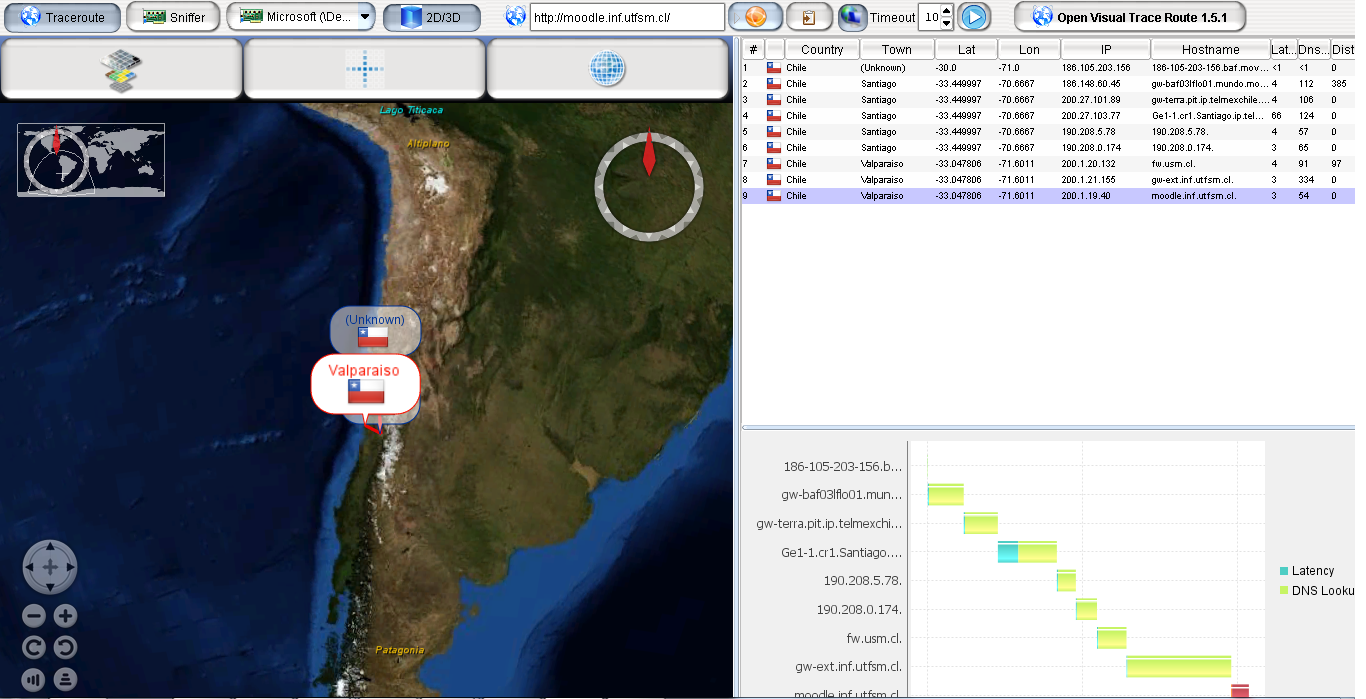
\includegraphics[width=0.9\textwidth]{pantalla1.png} 
\caption{http://moodle.inf.utfsm.cl/}
\end{center}
\end{figure}

\begin{figure}[!ht]  
\begin{center} 
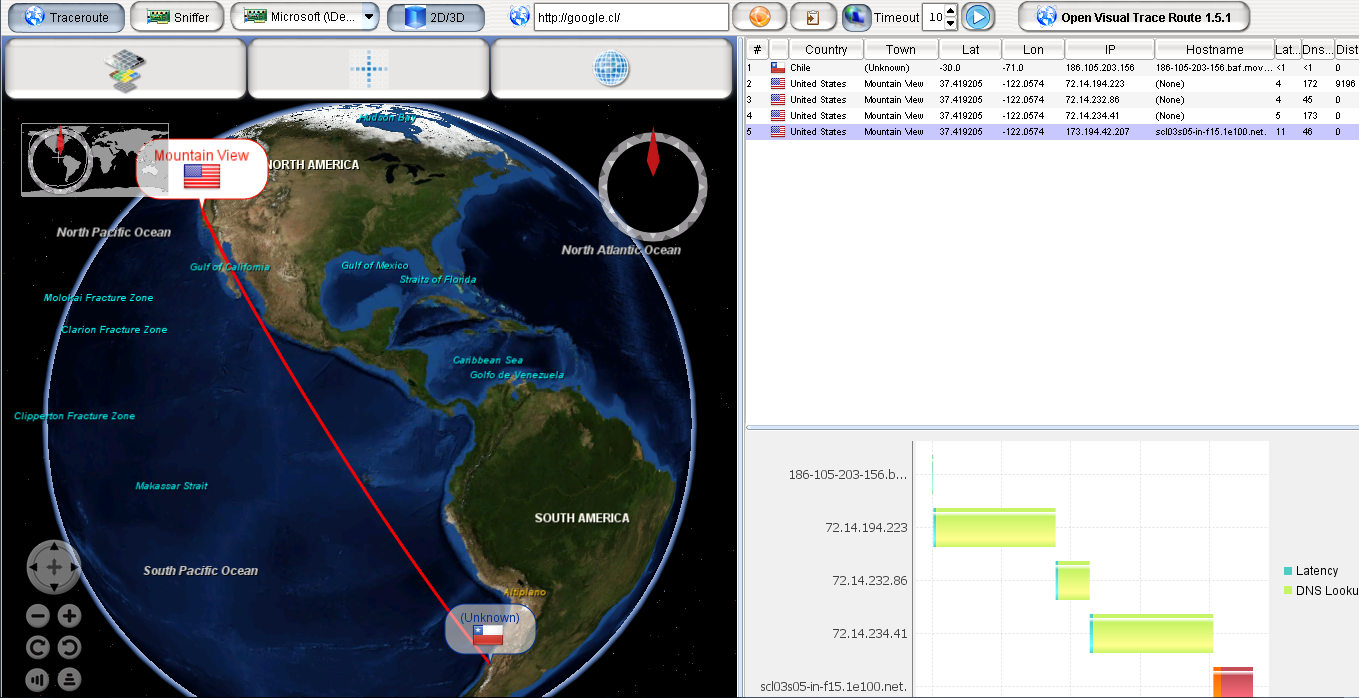
\includegraphics[width=0.9\textwidth]{pantalla2.png} 
\caption{http://google.cl/}
\end{center}
\end{figure}

\begin{figure}[!ht]  
\begin{center} 
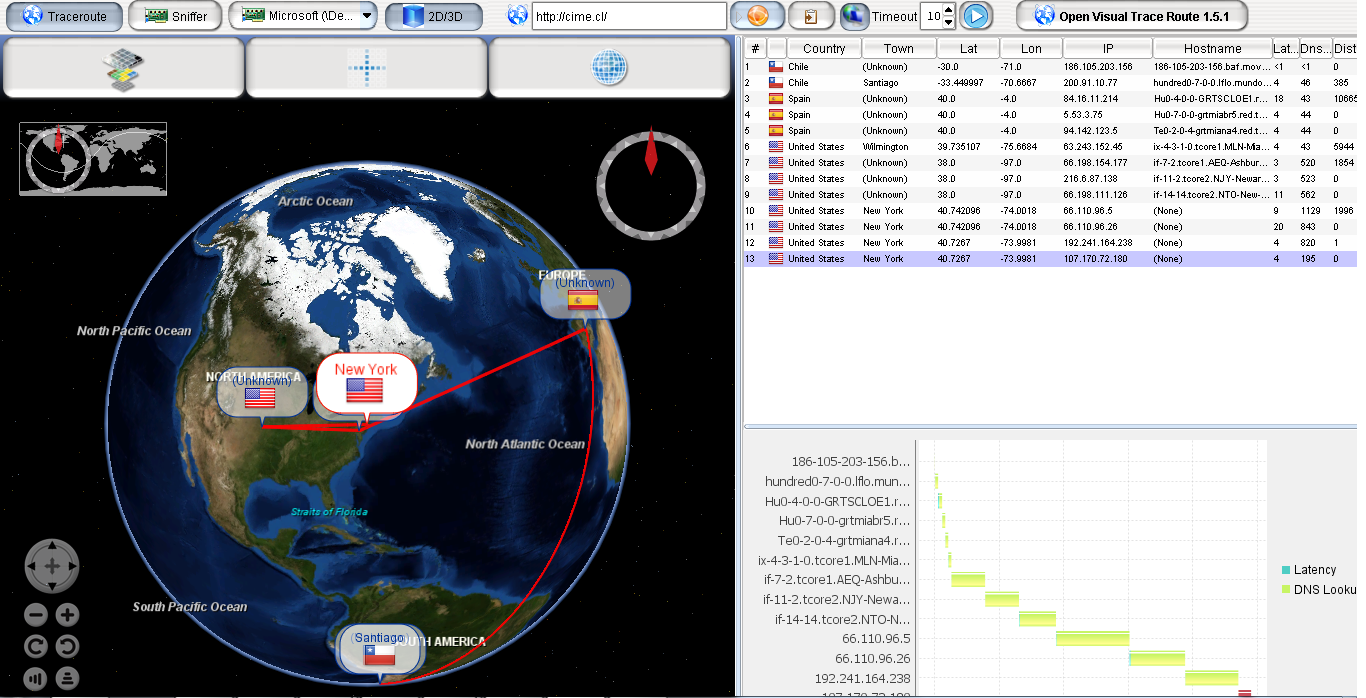
\includegraphics[width=0.9\textwidth]{pantalla3.png} 
\caption{http://cime.cl/}
\end{center}
\end{figure}

\begin{figure}[!ht]  
\begin{center} 
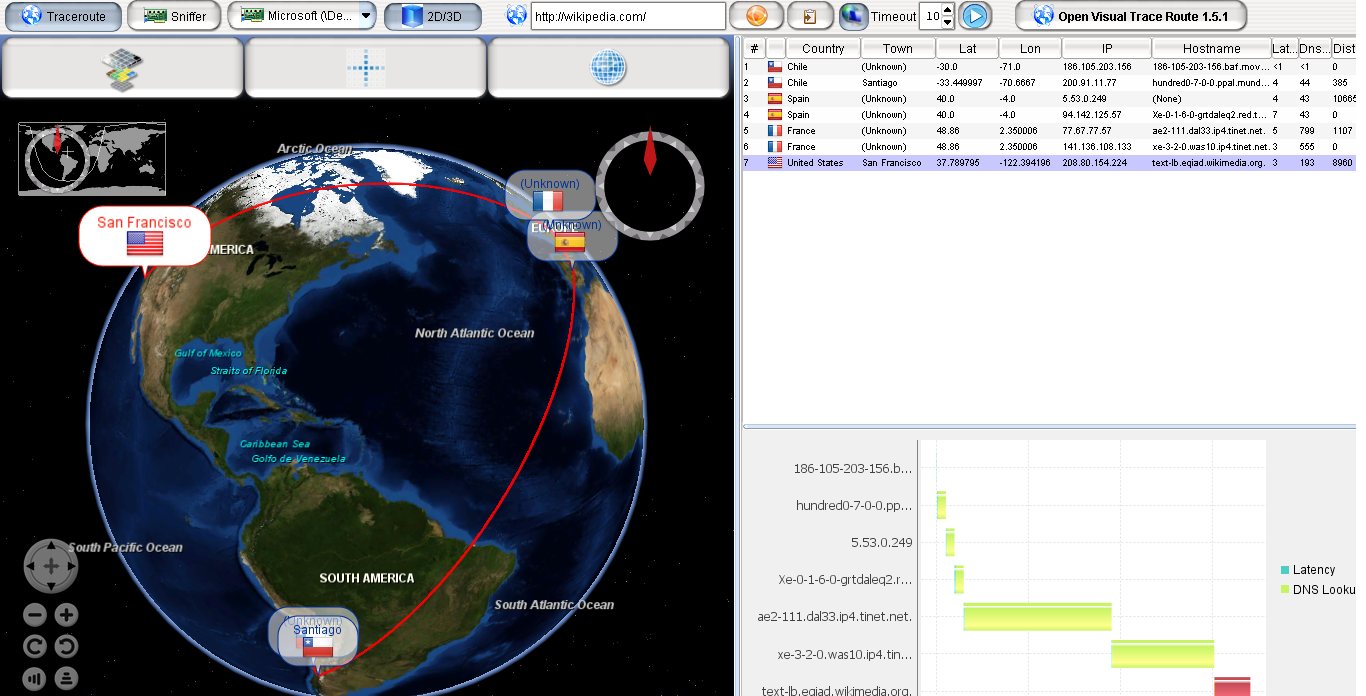
\includegraphics[width=0.9\textwidth]{pantalla4.png} 
\caption{http://wikipedia.com/}
\end{center}
\end{figure}

\begin{figure}[!ht]  
\begin{center} 
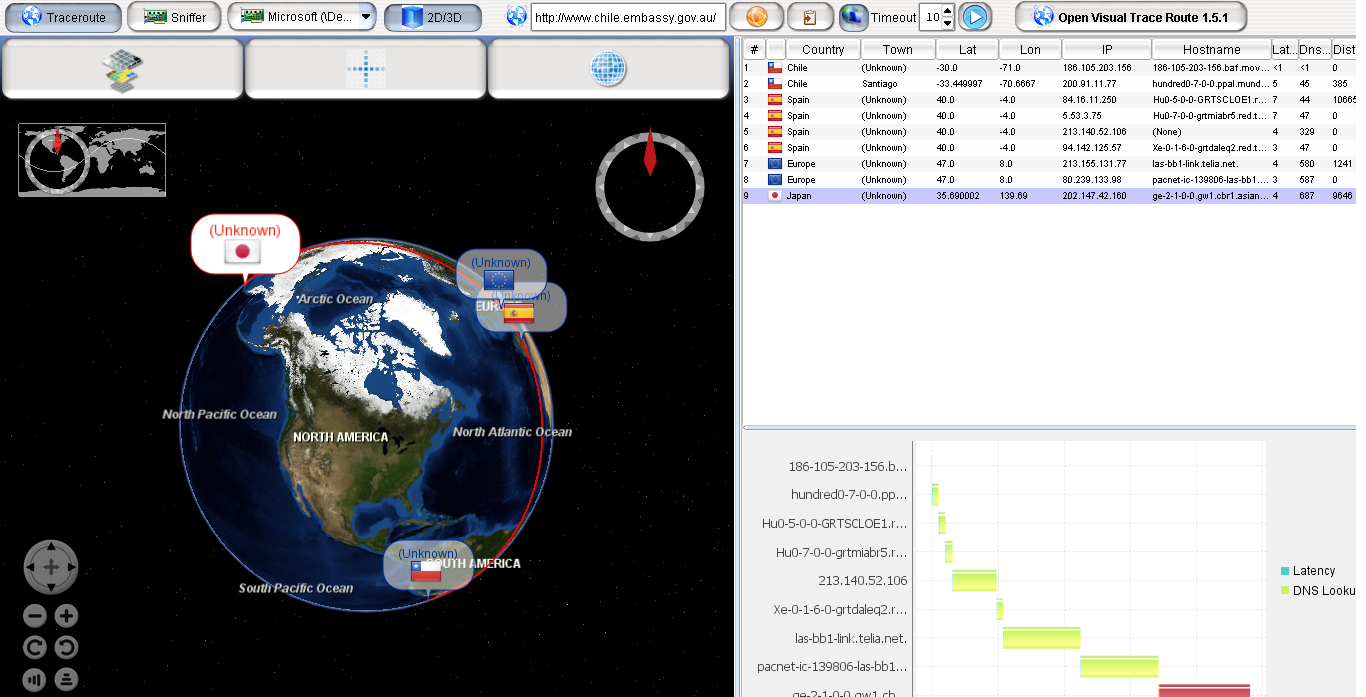
\includegraphics[width=0.9\textwidth]{pantalla5.png} 
\caption{http://www.chile.embassy.gov.au/}
\end{center}
\end{figure}

\item Pregunta 1 y 2 de Distancia Vector\\
\begin{figure}[!ht]  
\begin{center} 
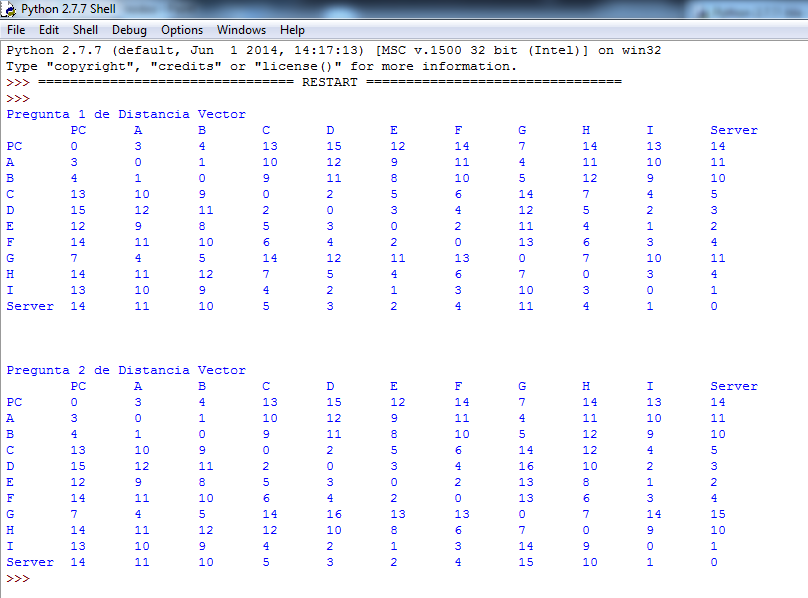
\includegraphics[width=0.9\textwidth]{nodos.png} 
\caption{Distancia Vector}
\end{center}
\end{figure}


\end{enumerate}
 
\end{document}